\documentclass[10pt]{article}

\usepackage[utf8]{inputenc} %Prise en charge des accents
\usepackage{csquotes}
\usepackage[english, french]{babel} %Charge les langues
\usepackage{color} %Charge les couleurs
\usepackage{fancyhdr} %Utilisation des entêtes
\usepackage{lastpage} %Script pour avoir le nombre de pages
\usepackage{graphicx} %Permet d'inclure des images
%\usepackage{makeidx} 
\usepackage{amsmath}
\usepackage{xspace} %Espaces intelligents
\usepackage{caption}
\usepackage{subfig}
\usepackage{multirow}
\usepackage{tabularx}
%\usepackage{picins} %Permet de faire des sous-figures
\usepackage{tikz} %Permet de dessiner
\usepackage[backend=bibtex]{biblatex}
\addbibresource{papers.bib}

\author{Léo \textsc{Baudouin}}
\title{Avancement Thèse}

\begin{document}

%\maketitle
\begin{center}
\begin{Huge}
Avancement Thèse
\end{Huge}

\vspace{3mm}
\begin{Large}
Léo \textsc{Baudouin}
\end{Large}

\vspace{3mm}
\today
\end{center}


\section{Vision}
\subsection{Vision classique}

A partir du livre de \citeauthor{Hartley03Book} \citetitle{Hartley03Book}, j'ai écrit les fonctions en C++ (avec OpenCV) nécessaire pour la reconstruction 3D.
C'est à dire : 
\begin{itemize}
\item RANSAC
\item Triangulation
\item Calcul de la matrice Fondamentale/Essentielle
\item Extraction des matrices $\mathbf{R}$ et $\mathbf{t}$
\item Ajustement de faisceaux
\end{itemize}
J'ai essayé plusieurs solutions lorsque c'était possible (SVD, pseudo-inverse, Levenberg-Marquardt, \dots), ou plusieurs méthodes (triangulation).
J'ai essayé également le tenseur trifocal sans succès.

J'obtiens des résultats satisfaisant à partir d'images simulées :
\begin{figure}[ht]
\begin{center}
\subfloat[Nuage simulé]{\label{fig:create}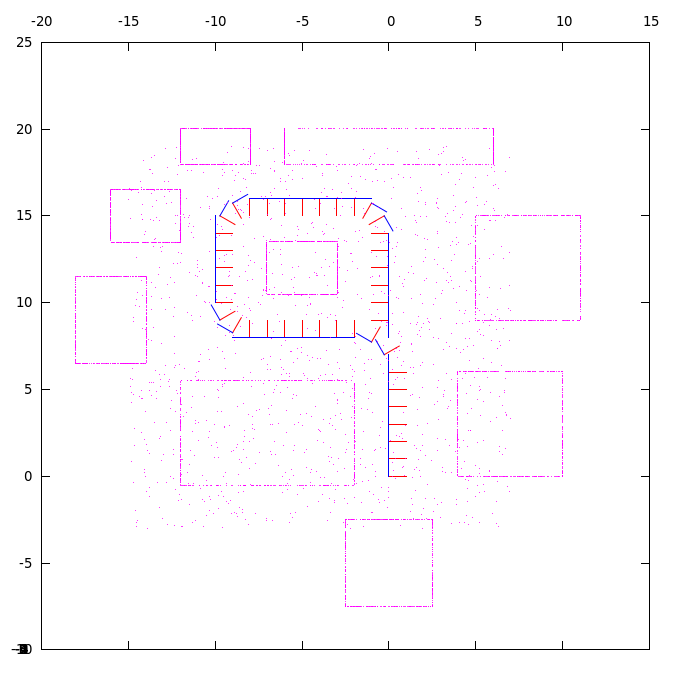
\includegraphics[width=0.45\linewidth]{images/createimage.png}}
\subfloat[Nuage recréé]{\label{fig:build}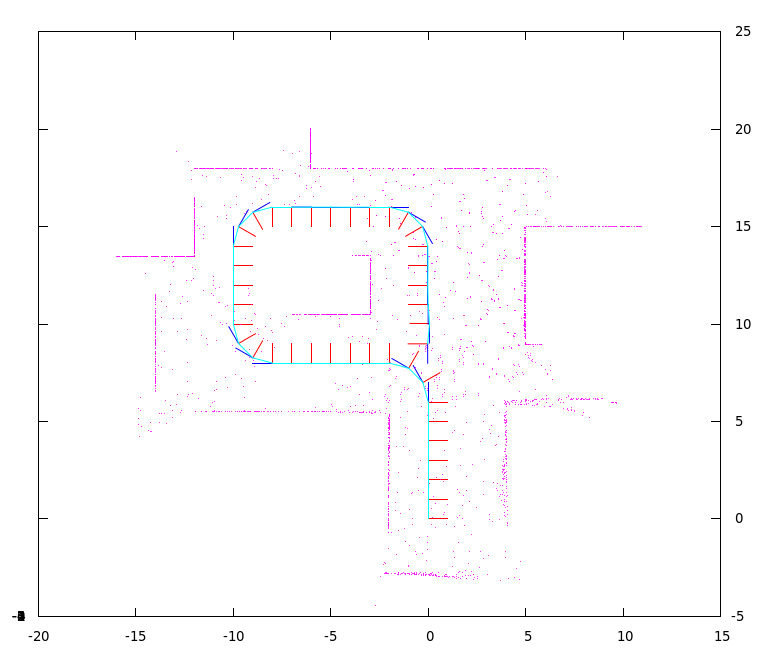
\includegraphics[width=0.45\linewidth]{images/buildfromvideo.png}}
\caption{L'image~\ref{fig:create} représente le nuage de points simulé ainsi que les différentes prises de vues, l'axe de la caméra ($\vec{z}$) est en bleu. Dans l'image~\ref{fig:build} on peut voir le résultat obtenu lors de la création du nuage à partir des images précédemment simulées.}
\end{center}
\end{figure}

\subsection{Vision Omnidirectionnelle}

J'ai écrit les mêmes fonctions dans le cas omnidirectionnelle.
Cependant j'ai des problèmes à estimer correctement $\mathbf{R}$ et $\mathbf{t}$ entre deux vues successives.
La méthode présentée dans \citetitle{Puig11PhD} de \citeauthor{Puig11PhD} a été implémentée.
Celle ci donne de bons résultats quand la caméra se déplace en ligne droite mais dès qu'elle tourne, l'algorithme ne converge plus vers la solution.

\subsection{SoViN}

J'ai testé la librairie SoViN, mais je n'ai pas encore pu l'utiliser au sein de mon programme. Pour l'instant SoViN est fait pour fonctionner de manière autonome, en utilisant une interface conçue par J.~\textsc{Courbon}.
Je viens juste d'avoir la version 2.0, et je vais essayer de participer au développement afin d'implémenter de nouvelles fonctions utiles dans le cadre de ma thèse.

\section{Navigation}

J'ai lu de nombreux articles concernant la navigation de robot mobile utilisant des cartes pré-construites.
Je n'ai pas encore commencé à programmer cette partie, je vais commencer dans peu de temps.

\section{Conclusion}

Je sais que j'ai pris énormément de retard en reprogrammant les fonctions de base pour la vision.
Cependant j'avais besoin de comprendre réellement comment elles fonctionnaient.
L'échec de la reconstruction dans le cas omnidirectionnel est un problème majeur pour moi, car je n'ai pas réussi à trouver des librairies existante permettant de résoudre ce problème.
Sachant que le laboratoire utilise couramment ce genre de fonctions, j'espère pouvoir trouver rapidement ce que je recherche.

En attendant je vais continuer de travailler avec des nuages de points simulés pour mettre en place des algorithmes de navigation et de mise en formation de flotte de robots.

\end{document}
